\chapter{Navier-Stokes equation -- Laminar compressible flow over a step}

\modinfo{Directory}{FlowStepCompressible}
\modinfo{Solvers}{\Idx{HeatSolve}, \Idx{FlowSolve}}
\modinfo{Tools}{\Idx{ElmerGUI}}
\modinfo{Dimensions}{2D, Steady-state}
\modinfo{Author}{Juha Ruokolainen, Rich Bayless}


\subsection*{Case definition}

This tutorial demonstrates how to simulate compressible air flowing past a step. The whole step has length of 1.4 m and the height of 0.2 m and the first part of it has length of 0.4 m and the height of 0.1 m (Figure \ref{fg:step_geometry}). The model has three sets of boundary conditions. The air flows into the step from the inlet region and withdraws from the outlet region. The other edges of the step compose the third boundary.\\

\begin{wrapfigure}{r}{0.2\textwidth}
\begin{displaymath}
\rho = \frac{p}{RT},
\end{displaymath}
\end{wrapfigure}

The flowing air is considered as an ideal gas in this case, and its density $\rho$  depends on the pressure $p$ and temperature $T$ through the equation of state where $R$ is the gas constant.  The following table lists the material parameters for the gas used in this tutorial.  Note that the parameters being used in this tutorial are different from the parameters that would be retrieved from the Material Library, if one selected the entry for `Air (Room Temperature).\\

\begin{table}[h]
\caption{Material parameters.}
\label{tb:matpam}
\begin{center}
\begin{tabular}{ll} \hline
parameter  & value \\ \hline
viscosity & 16.7e-6 Ns/m$^{2}$  \\
heat conductivity & 0.026 W/(m$\cdot$K) \\
heat capacity & 1.01e3 J/(kg$\cdot$K) \\
specific heat ratio & 1.4        \\
reference pressure & 1e5 Pa      \\ \hline
\end{tabular}
\end{center}
\end{table}

The geometry looks as shown in figure \ref{fg:step_geometry} 

\begin{figure}[H]
\centering
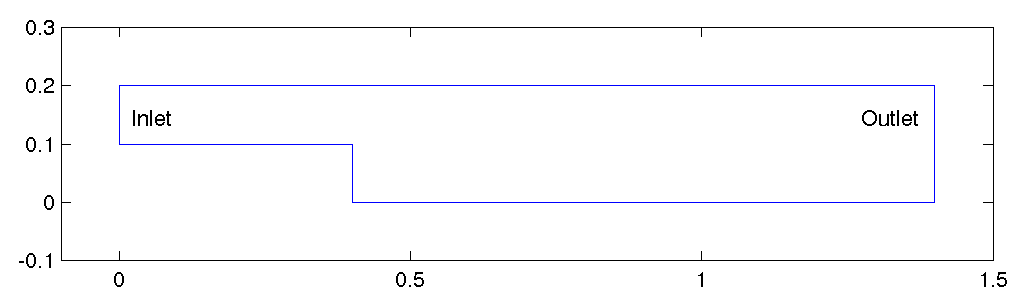
\includegraphics[width=0.8\textwidth]{step_geometry.png}
\caption{Geometry of the Step.}\label{fg:step_geometry}
\end{figure}  

\subsection*{Check ElmerGUI Equation Menu}

We will be using the \Idx{FlowSolver} and the \Idx{HeatSolver}, which are the default, pre-loaded GUI definitions, so they don't need to be manually activated.  For reference, the  \texttt{\Idx{heatequation.xml}} and \texttt{\Idx{navier-stokes.xml}} definition files are, by default, located in Linux in:

\texttt{\$ELMER\_HOME/share/ElmerGUI/edf}\\

and in Windows, located in:

\texttt{C:/Program Files/Elmer 9.0-Release/share/ElmerGUI/edf}\\

\subsection*{Solution procedure}

The mesh is given in ElmerGrid format in file \texttt{mesh.grd}, load this file.
\ttbegin
File 
  Open -> mesh.grd
\ttend

You should obtain your mesh and may check \texttt{Model Summary...} that it consists of 531 surface elements.  Your mesh should look like as shown in figure \ref{fg:step_mesh}.

\begin{figure}[H]
\centering
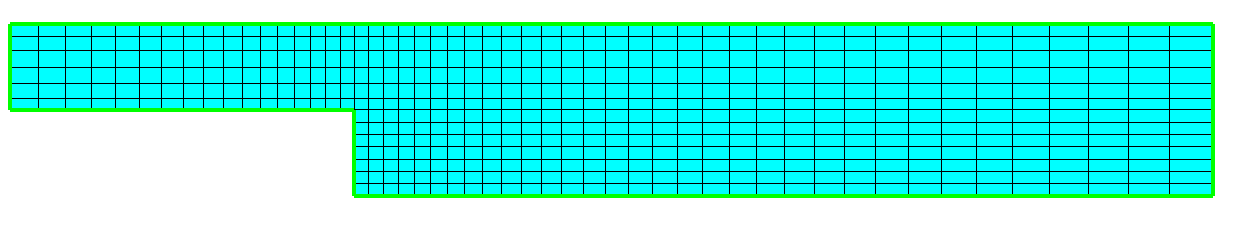
\includegraphics[width=0.8\textwidth]{step_mesh}
\caption{Mesh}\label{fg:step_mesh}
\end{figure}  

After we have the mesh we start to go through the Model menu from the top to bottom. In the Setup we choose things related to the whole simulation such as file names, 
time stepping, constants etc. The simulation uses 2D Cartesian geometry and the problem is solved in steady state using no more than twenty steady state iterations.

\ttbegin
Model
  Setup 
    Simulation Type = Steady State
    Steady state max. iter = 20
  Apply
\ttend

In the equation section we choose the relevant equations and parameters related to their solution. 

In this case we'll have one set of equations (named ``Heat and Flow'') which consists of the Heat equation and of the Navier-Stokes equation.

When defining Equations and Materials it is possible to assign to the bodies immediately, or to use mouse selection to assign them later. In this case we have just one body and therefore its easier to assign the Equation and Material to it directly.  It is important to select the convection to be computed since that couples the velocity field to the heat equation.\\

For the linear system solvers we are happy to use the defaults. One may however, try out different preconditioners (ILU1,\ldots) or direct Umfpack solver, for example.

\ttbegin
Model
  Equation
   Name = Heat and Flow
    Apply to Bodies = 1
    Heat Equation
      Active = on
      Convection = Computed
        Edit Solver Settings
           General
             Numerical techniques
                Stabilize = uncheck
                Bubbles  = check
          Apply (to exit Edit Solver Settings)
    Navier-Stokes
      Active = on
        Edit Solver Settings
           General
             Numerical techniques
                Stabilize = uncheck
                Bubbles  = check
          Apply (to exit Edit Solver Settings)
    Add 
    OK
\ttend        

The Material section includes all the material parameters. They are divided into generic parameters which are direct properties of the material without making any assumptions on the physical model, such as the mass. Other properties assume a physical law, such as conductivities and viscosity.\\

Our intention is to model compressible flow and that is why we have to set the value ''Perfect Gas'' for the {\tt Compressibility Model} entry. Furthermore, because perfect gas model has been chosen the settings {\tt Reference Pressure} and {\tt Specific Heat Ratio} must also be given. The Navier-Stokes equation also needs the value of viscosity and the heat equation needs the values of heat capacity and heat conductivity.  We will not use the Material Library, instead we will enter our own values.  The needed material parameters for an ideal gas for this tutorial are listed in table \ref{tb:matpam}.

\ttbegin
Model
  Material
   Name = Our Ideal Gas
    Apply to Bodies = 1 
    General
      Heat Capacity = 1.01e3
      Specific Heat Ratio = 1.4
      Reference Pressure = 1.0e5
    Heat Equation
      Heat Conductivity = 0.026
    Navier-Stokes
       Viscosity = 16.7e-6
       Compressibility models = Perfect Gas
    Add
    OK
\ttend

A Body Force represents the right-hand-side of a equation. It is generally not a required field for a body.\\

Initial conditions should be given to transient cases, and probably are not needed for steady state solutions.  For the initial condition of temperature we have chosen 300 K.

\ttbegin
Model
  Initial Condition 
    Name = Initial Guess
    Apply to Bodies = 1 
    Heat Equation
      Temperature = 300
    Add 
    OK
\ttend

Only one boundary condition may be applied to each boundary and therefore all the different physical BCs for a boundary should be grouped together. 

There are three sets of boundary conditions, so three {\tt Boundary Condition} sections are needed. The first one is used to prescribe the boundary conditions in the inlet region. Note that we have defined the x-velocity and temperature as a variable of y-coordinate.  This is done by setting different values for the x-velocity and temperature (the numerical values of the second column between the words {\tt Real} and {\tt End}) in the different y-points (the numerical values of the first column between words {\tt Real} and {\tt End}) of the inlet region. This kind of procedure prevents singularities from occurring in the corner points of the inlet region. In addition, this kind of definition is more realistic than a constant condition, in which the values of the x-velocity and temperature remain the same in the whole inlet region.\\

To enter the three pairs of numbers in the Heat Equation menu tab, click into the box labelled Temperature under Dirichlet Conditions, then press the enter key.  An editor window will pop up and you can enter all of the text from `Temperature' to `Navier-Stokes' into the window.  Repeat the same steps in the Navier-Stokes menu tab, and enter all the text from `Velocity 1' to `Velocity 2'.    Refer to Figure\ref{fg:bc}, where the left side shows the Temperature boundary condition for Heat and the right side shows the Velocity 1 boundary condition for Flow.

\begin{figure}[H]
\centering
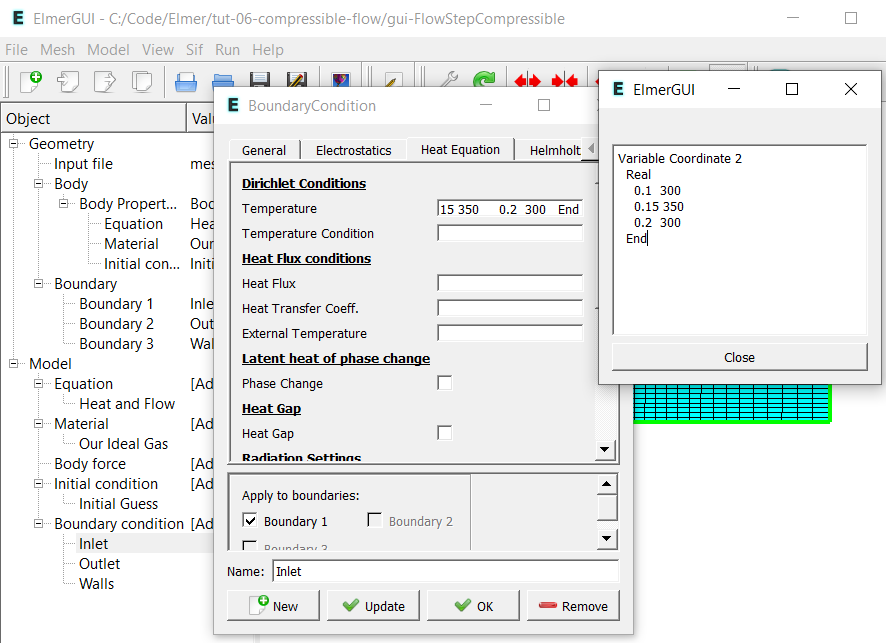
\includegraphics[width=0.48\textwidth]{bc-heat}
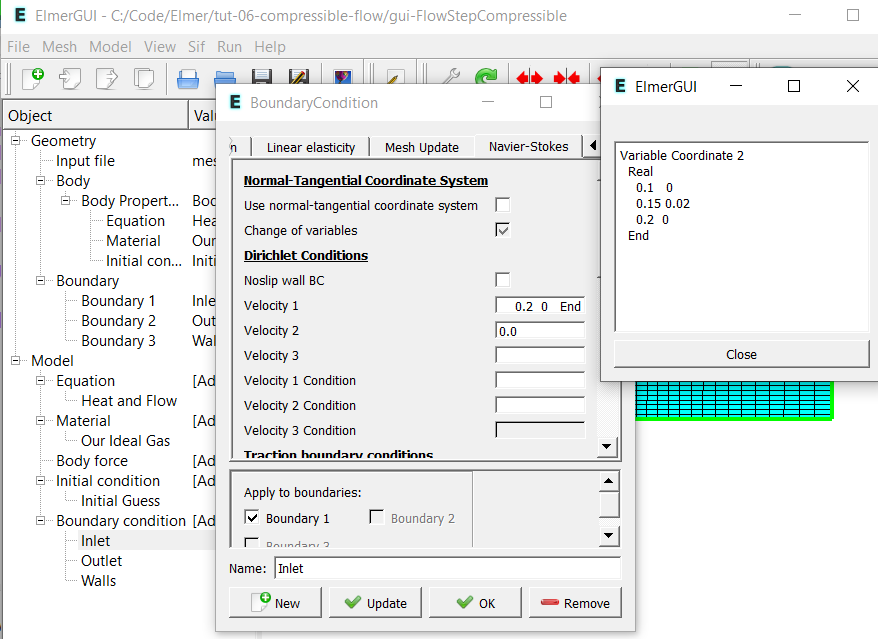
\includegraphics[width=0.48\textwidth]{bc-flow}
\caption{Left side: Heat BC, Right side: Flow BC}\label{fg:bc}
\end{figure}  

\newpage

\ttbegin
Model
  BoundaryCondition
    Name = Inlet
    Heat Equation
      Temperature = Variable Coordinate 2
         Real 
           0.1    300
           0.15   350
           0.2    300
        End
    Navier-Stokes 
      Velocity 1 = Variable Coordinate 2
           Real 
             0.1    0
            0.15   0.02
            0.2    0
         End
      Velocity 2 = 0.0
    Add
    New
\ttend

After the rest of the boundary conditions have been defined the problem is ready to solve.

\ttbegin
    Name = Outlet
    Navier-Stokes 
      Velocity 2 = 0.0
    Add 
    New
 
    Name = Walls
    Heat Equation
       Temperature = 300
    Navier-Stokes 
      Noslip wall BC = on
    Add
    OK
\ttend   

The conditions may also be assigned to boundaries in the Boundary condition menu, or by clicking on each boundary with the mouse. Here we use the latter approach as that spares us of the need to know the indexes of each boundary.

\ttbegin
Model
  Set boundary properties
    Choose Inlet -> set boundary condition
    Choose Outlet -> set boundary condition
    Choose Walls -> set boundary condition
   OK 
\ttend


For the execution ElmerSolver needs the mesh files and the command file.  We have now basically defined all the information for ElmerGUI to write the command file. After writing it we may also visually inspect the command file.

\ttbegin
Sif 
  Generate
  Edit -> look how your command file came out  
\ttend

Before we can execute the solver we should save the files in a directory. The ElmerGUI project includes all the files needed to restart the case.

\ttbegin
File 
  Save Project
\ttend

After we have successfully saved the files we may start the solver

\ttbegin
Run
  Start solver
\ttend
A convergence view automatically pops up showing relative changes of each iteration.

When there are some results to view we may start the postprocessor also

\ttbegin
Run
  Start ParaView
\ttend


\subsection*{Results}

The simulation may take about a minute.  You may inspect the results with Paraview.\\

\begin{figure}[H]
\centering
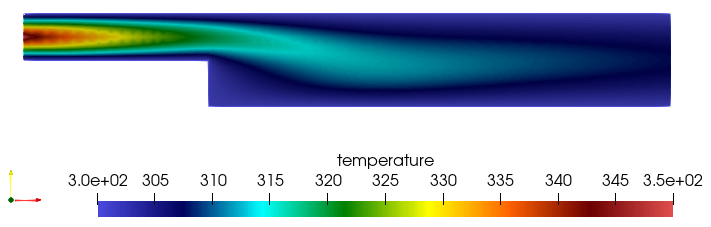
\includegraphics[width=0.9\textwidth]{temperature}
\caption{Temperature distribution}\label{fg:temp}
\end{figure} 

\begin{figure}[H]
\centering
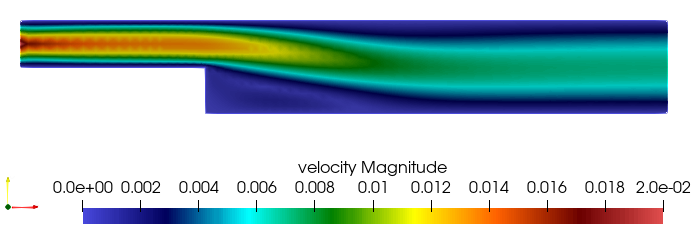
\includegraphics[width=0.9\textwidth]{velocity}
\caption{Velocity distribution}\label{fg:velocity}
\end{figure} 

\begin{figure}[H]
\centering
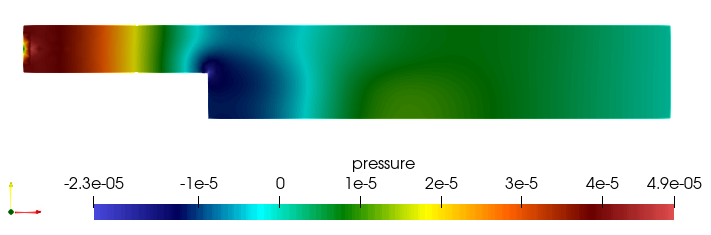
\includegraphics[width=0.9\textwidth]{pressure}
\caption{Pressure distribution}\label{fg:pressure}
\end{figure} 



\subsection*{Extra task:}

If you have time you may try to solve the case with different parameters, such as doubling the peak inlet velocity in the inlet boundary condition from 0.02 to 0.04.  See how much you can increase the peak inlet velocity and still converge to a solution.

\hfill
